\documentclass[tikz]{standalone}
\usepackage[blue]{causets}
\usetikzlibrary{fit,shapes.geometric}
\begin{document}
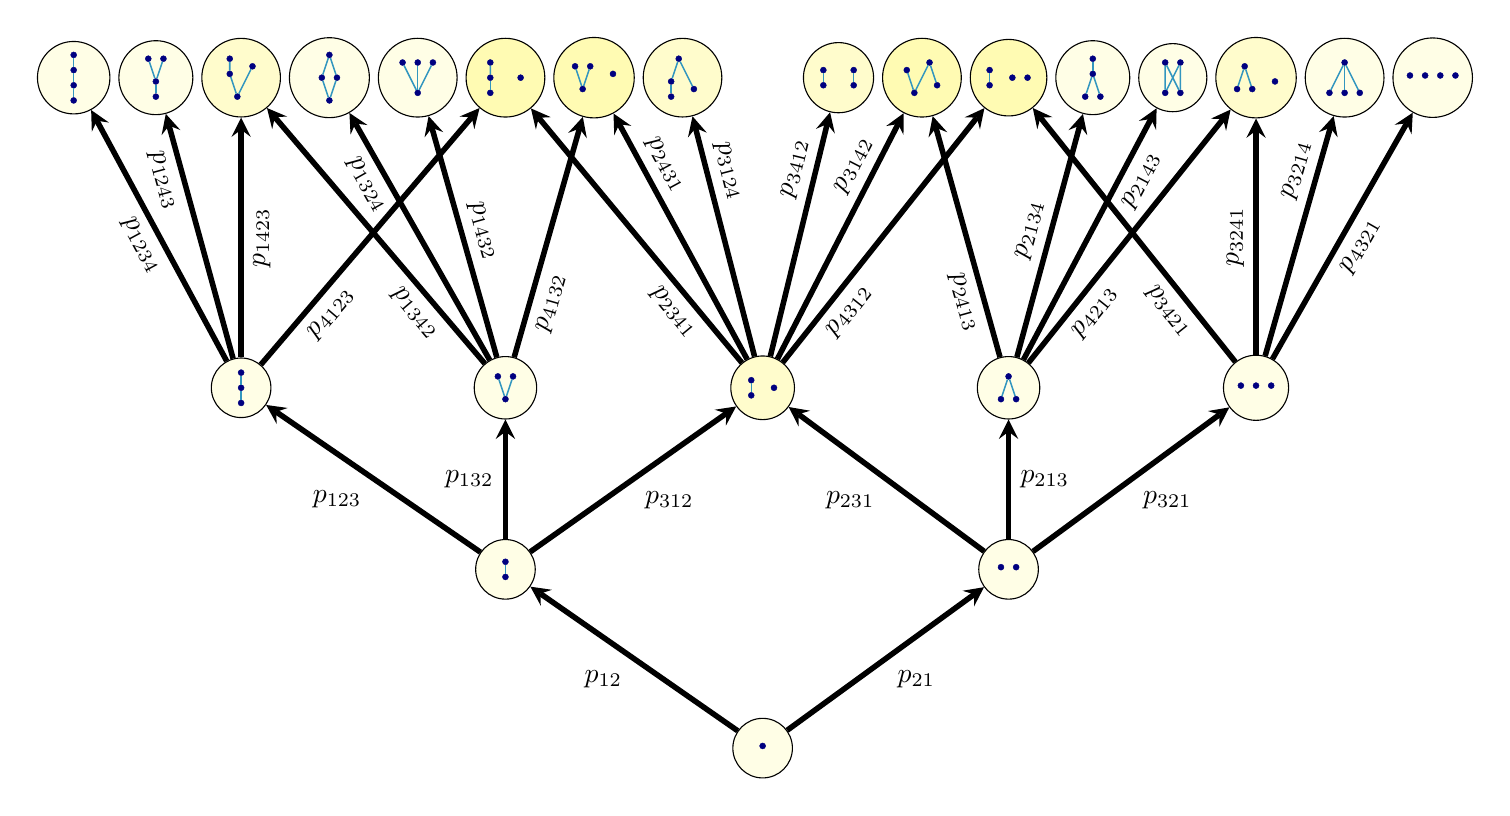
\begin{tikzpicture}[-stealth, line width=2pt]
	\matrix[nodes={draw, fill=yellow!10, thin, circle, inner sep=0.6ex, minimum size=5ex}, row sep=1.5cm, column sep=0.1cm]
	{
		\node (C1234) {\pcauset{1,2,3,4}}; 
	& \node (C1243) {\pcauset{1,2,4,3}}; 
	& \node[fill=yellow!20] (C1423) {\pcauset{1,4,2,3}}; 
	& \node (C1324) {\pcauset{1,3,2,4}}; 
	& \node (C1432) {\pcauset{1,4,3,2}}; 
	& \node[fill=yellow!30] (C4123) {\pcauset{4,1,2,3}}; 
	& \node[fill=yellow!30] (C4132) {\pcauset{4,1,3,2}}; 
	& \node[fill=yellow!20] (C3124) {\pcauset{3,1,2,4}}; 
	& & \node[fill=yellow!20] (C3412) {\pcauset{3,4,1,2}}; 
	& \node[fill=yellow!30] (C3142) {\pcauset{3,1,4,2}}; 
	& \node[fill=yellow!30] (C4312) {\pcauset{4,3,1,2}}; 
	& \node (C2134) {\pcauset{2,1,3,4}}; 
	& \node (C2143) {\pcauset{2,1,4,3}}; 
	& \node[fill=yellow!20] (C4213) {\pcauset{4,2,1,3}}; 
	& \node (C3214) {\pcauset{3,2,1,4}}; 
	& \node (C4321) {\pcauset{4,3,2,1}}; 
	\\
	\\
	& & \node (C123) {\pcauset{1,2,3}}; 
	& & & \node (C132) {\pcauset{1,3,2}}; 
	& & & \node[fill=yellow!20] (C312) {\pcauset{3,1,2}}; 
	& & & \node (C213) {\pcauset{2,1,3}}; 
	& & & \node (C321) {\pcauset{3,2,1}}; 
	\\
	& & & & & \node (C12) {\pcauset{1,2}}; 
	& & & & & & \node (C21) {\pcauset{2,1}}; 
	\\
	& & & & & & & & \node (C1) {\pcauset{1}}; 
	\\
	};
	\draw (C1) -- node[below left] {$p_{12}$} (C12);
	\draw (C12) -- node[below left] {$p_{123}$} (C123);
	\draw (C123) -- node[sloped, midway, below] {$p_{1234}$} (C1234);
	\draw (C123) -- node[sloped, near end, below] {$p_{1243}$} (C1243);
	\draw (C123) -- node[sloped, midway, below] {$p_{1423}$} (C1423);
	\draw (C123) -- node[sloped, near start, below] {$p_{4123}$} (C4123);
	\draw (C12) -- node[left] {$p_{132}$} (C132);
	\draw (C132) -- node[sloped, near start, below] {$p_{1342}$} (C1423);
	\draw (C132) -- node[sloped, near end, below] {$p_{1324}$} (C1324);
	\draw (C132) -- node[sloped, midway, above] {$p_{1432}$} (C1432);
	\draw (C132) -- node[sloped, near start, below] {$p_{4132}$} (C4132);
	\draw (C12) -- node[below right] {$p_{312}$} (C312);
	\draw (C312) -- node[sloped, near end, above] {$p_{3124}$} (C3124);
	\draw (C312) -- node[sloped, near end, above] {$p_{3412}$} (C3412);
	\draw (C312) -- node[sloped, near end, above] {$p_{3142}$} (C3142);
	\draw (C312) -- node[sloped, near start, below] {$p_{4312}$} (C4312);
	\draw (C1) -- node[below right] {$p_{21}$} (C21);
	\draw (C21) -- node[below left] {$p_{231}$} (C312);
	\draw (C312) -- node[sloped, near start, below] {$p_{2341}$} (C4123);
	\draw (C312) -- node[sloped, near end, above] {$p_{2431}$} (C4132);
	\draw (C21) -- node[right] {$p_{213}$} (C213);
	\draw (C213) -- node[sloped, midway, above] {$p_{2134}$} (C2134);
	\draw (C213) -- node[sloped, near start, below] {$p_{2413}$} (C3142);
	\draw (C213) -- node[sloped, near end, below] {$p_{2143}$} (C2143);
	\draw (C213) -- node[sloped, near start, below] {$p_{4213}$} (C4213);
	\draw (C21) -- node[below right] {$p_{321}$} (C321);
	\draw (C321) -- node[sloped, near start, below] {$p_{3421}$} (C4312);
	\draw (C321) -- node[sloped, midway, above] {$p_{3241}$} (C4213);
	\draw (C321) -- node[sloped, near end, above] {$p_{3214}$} (C3214);
	\draw (C321) -- node[sloped, midway, below] {$p_{4321}$} (C4321);
\end{tikzpicture}
\end{document}
